

\section{AdHoc Problems}

\begin{frame}
  \centering
  {\huge
    Week 1 -- Part 3: AdHoc Problems
  }
\end{frame}

\begin{frame}
  \frametitle{Today's Class: Ad Hoc Problems}

  \begin{itemize}
  \item \structure{Ad Hoc}: Problems that don't have a single algorithm;
  \bigskip

  \item Common forms of Input and Output
  \bigskip

  \item Debugging and Creating Test Cases
  \bigskip

  \item Some Problem Analysis
  \end{itemize}

\end{frame}

\section{Problem Analysis: 3n+1}
\subsection{Wrong Answer}
\begin{frame}[fragile]
  \frametitle{Reading the Problem: 3n+1}

  \begin{block}{}
    For any two numbers $i$ and $j$, calculate the \structure{Maximum Cycle Length}.
  \end{block}

  \bigskip

\begin{verbatim}
Algorithm A(n)
1. print n
2. if n == 1 then STOP
3. if n is odd then n = 3n + 1
4. else n = n/2
5. GOTO 2


Example: A(22)
22 11 34 17 52 26 13 40 20 10 5 16 8 4 2 1

Size: 16
\end{verbatim}
\end{frame}

\begin{frame}[fragile]
  \frametitle{Problem 3n+1 -- Solution 1}
\begin{verbatim}
while true:
  try:
    line = input()
    max = 0
    tk = line.split()
    i, j = int(tk[0]), int(tk[1])
    for n in range(i, j+1):
      count = 1
      while n != 1:
        if n % 2 == 1: x = 3 * x + 1
        else: n = n / 2
        count += 1
      if count > max: max = count
      print (line, max)
  except EOFError: break
\end{verbatim}
\end{frame}

\begin{frame}
  \frametitle{Solution 1: Problem!}

  \begin{itemize}
    \item Solution 1 solves all \structure{Sample Input} correctly.
    \bigskip

    \item But we still get \alert{Wrong Answer!}
    \bigskip

    \item Why??? :-(
  \end{itemize}
\end{frame}

\begin{frame}[fragile]
  \frametitle{Solution 1: Traps!}

  \begin{itemize}
    \item Solution 1 solves all \structure{Sample Input} correctly.
    \bigskip

    \item If we try the input: \alert{20 10} -- output is \alert{nothing!}
\begin{verbatim}
for x in range(i, j+1):   <-- Error is here!
  ...
  print (line, max)
\end{verbatim}
    \bigskip

    \item The sample input has \alert{no examples} with "\alert{$i > j$}"!
  \end{itemize}
\end{frame}

\begin{frame}
  \frametitle{Solution 1: Traps!}

    \begin{block}{Input Description}
    The input will consist of a series of \alert{pairs of integers} i and j, one pair of
    integers per line. All integers will be \alert{less than 10,000 and greater than 0.}

    \bigskip

    You should process all pairs of integers and for each pair determine the maximum
    cycle length over \alert{all integers between and including i and j}.

    \bigskip

    You can \alert{assume that no operation overflows a 32-bit integer}.
    \end{block}
    \bigskip

    The only rules are those \structure{expressely written!}
\end{frame}

\begin{frame}
  \frametitle{Solution 1: Traps!!!!!}

  \begin{itemize}
    \item First rule of Programming Challenges: \\ \hspace{1cm}\alert{Assume Worst Case}
    \item Always try the worst case input!

    \bigskip

    \begin{itemize}
      \item Number is Negative; Number is zero;
      \item Number is out of order (or in order);
      \item Number is repeated;
      \smallskip

      \item Graph is unconnected; Graph is Fully connected;
      \item Lines are parallel; Points are in the same place;
      \item Area is 0; Angle is 0;
      \smallskip

      \item Input is very long;
      \item Input is very short;
    \end{itemize}
    \bigskip

    \item If it is not against the rules: \alert{It will happen!}
    \item This also happens in programs in the real world.
  \end{itemize}
\end{frame}

\subsection{Time Limited Exceeded}

\begin{frame}[fragile]
  \frametitle{Problem 3n+1 -- Solution 2}
\begin{verbatim}
while true:
  try:
    line = input()
    max = 0
    tk = line.split()
    i, j = int(tk[0]), int(tk[1])
    for n in range(min(i, j), max(i, j)+1): # FIXED!
      count = 0
      while n != 1:
        if n % 2 == 1: n = 3 * n + 1
        else: n = n / 2
        count += 1
      if count > max: max = count
      print (line, max)
  except EOFError: break
\end{verbatim}
\end{frame}

\begin{frame}
  \frametitle{Solution 2: Time Limited Exceeded!}
  \begin{itemize}
    \item All the inputs are correct.
    \bigskip

    \item But now we have \alert{Time Limited Exceeded}
    \bigskip

    \item Why?
  \end{itemize}
\end{frame}

\begin{frame}[fragile]
  \frametitle{Solution 2: Cost Calculation}

    \begin{block}{Input Description}
    All integers will be \alert{less than 10,000 and greater than 0.}
    \bigskip

    You can \alert{assume that no operation overflows a 32-bit integer}.
    \end{block}
    \bigskip

    \begin{itemize}
      \item What happens when the input is \structure{1 10000}?
\begin{verbatim}
1 10000 262
\end{verbatim}
      \bigskip

      \item The longest sequence in 1, 10000 has 262 steps.
      \item But we calculate \alert{all} sequences between 1, 10000.
      \item Worst case: 10000*262 = 2,000,000 steps!
      \bigskip

      \item For only one query!
    \end{itemize}
\end{frame}

\begin{frame}[fragile]
  \frametitle{Solution 2: Memoization}

  \begin{itemize}
    \item Let's think about A();
\begin{verbatim}
A(22):  22 11 34 17 52 26 13 40 20 10 5 16 8 4 2 1
A(11):  11 34 17 52 26 13 40 20 10 5 16 8 4 2 1
A(17):  17 52 26 13 40 20 10 5 16 8 4 2 1
A(13):  13 40 20 10 5 16 8 4 2 1
A(10):  10 5 16 8 4 2 1
A(8) :  8 4 2 1
\end{verbatim}
    \bigskip

    \item Do we need to \alert{Recalculate} every time we see a new number?
  \end{itemize}

  \begin{block}{Good Technique: Memoization}
    If we know that we will use a result again in the future,
    we should \alert{store this result in the memory}.
  \end{block}
\end{frame}

\begin{frame}[fragile]
  \frametitle{Solution 2: Memoization Idea}
\begin{verbatim}
  table = {}
  table[1] = 1

  def A(n):
    if n in table.keys():
      return table[n]
    else:
      if n % 2 == 1:
        table[n] = 1 + A(3*n + 1)
      else:
        table[n] = 1 + A(n/2)
    return table[n]
\end{verbatim}
\end{frame}

\section{How to Solve Problems}
\subsection{Programming Challenge Workflow}
\begin{frame}
  \frametitle{A Programming Challenge Workflow}

  \begin{center}
    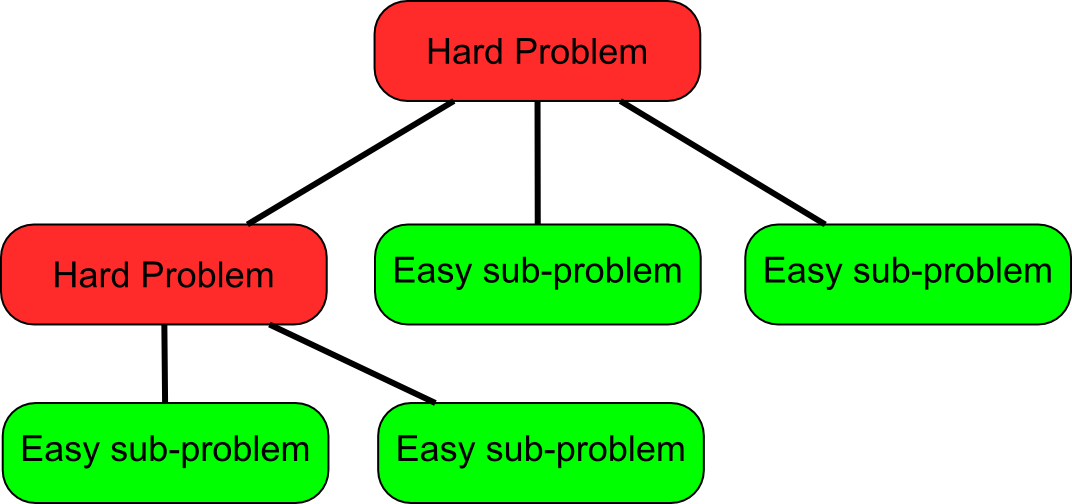
\includegraphics[width=0.5\textwidth]{../img/breakingtheproblem}
  \end{center}

  Trick to solve problems without bugs: Break the problem down
  \bigskip

  \begin{itemize}
  \item How to calculate the function $A()$;
  \item Imagine the worst possible cases ($i > j$);
  \item Calculate cost of solution;
  \item Improve speed with memoization;
  \end{itemize}
\end{frame}

\subsection{Programming Challenge Workflow}
\begin{frame}
  \frametitle{A Programming Challenge Workflow}

  Common Steps for Programming challenges:
  \bigskip

  \begin{itemize}
  \item Task 1: Read the problem description;
  \item Task 2: Read the input/output;
  \item Task 3: Think about the algorithm;
  \item Task 4: Write the Code;
  \item Task 5: Test the program on example data;
  \item Task 6: Test the program on hidden data;
  \end{itemize}
\end{frame}


\subsection{Task 1: Reading The Problem}
\begin{frame}
  \frametitle{Task 1: Understanding the Problem Description}

  The English description is so hard!

  \bigskip

  \begin{block}{Don't Worry:}
  \begin{enumerate}
  \item Separate the text into \structure{flavor} and \structure{rules};
  \item Sometimes it is easy to read the input/output first, and then
    the text;
  \item Problems with a lot of \structure{flavor} are usually not very hard.;
  \end{enumerate}
  \end{block}
\end{frame}

\begin{frame}
  \frametitle{Example: Problem 11559 -- Event Planning}

  {\smaller
  \begin{alertblock}{Flavor:}
    As you didn't show up to the yearly general meeting of the Nordic
    Club of Pin Collectors, you were unanimously elected to organize
    this years excursion to Pin City.  You are free to choose from a
    number of weekends this autumn, and have to find a suitable hotel
    to stay at, preferably as cheap as possible.
  \end{alertblock}

  \begin{exampleblock}{rules}
    You have some \structure{\underline{constraints}}: The total
    \structure{\underline{cost}} of the trip must be within
    \structure{\underline{budget}}, of course. All participants
    \structure{\underline{must}} stay at the same hotel, to avoid last years
    catastrophe, where some members got lost in the city, never being seen
    again.
  \end{exampleblock}}

  \bigskip

  {\bf Keywords:} constraints, minimum, maximum, cost, rules, number,
  etc...
\end{frame}

\begin{frame}
  \frametitle{Hints for hard to read problems}

  \begin{columns}
    \column{0.7\textwidth}
    {\small
    \begin{itemize}
    \item First, look at the \structure{sample input and output};
    \item Write the idea of the problem on paper
    \item Use the Paper: mark keywords;
    \item Use the Paper: cut flavor;
    \item \alert{Read the problem again!};
    \item \alert{Do not begin programming until you understand the problem!}
    \end{itemize}
    }
    \column{0.3\textwidth}
    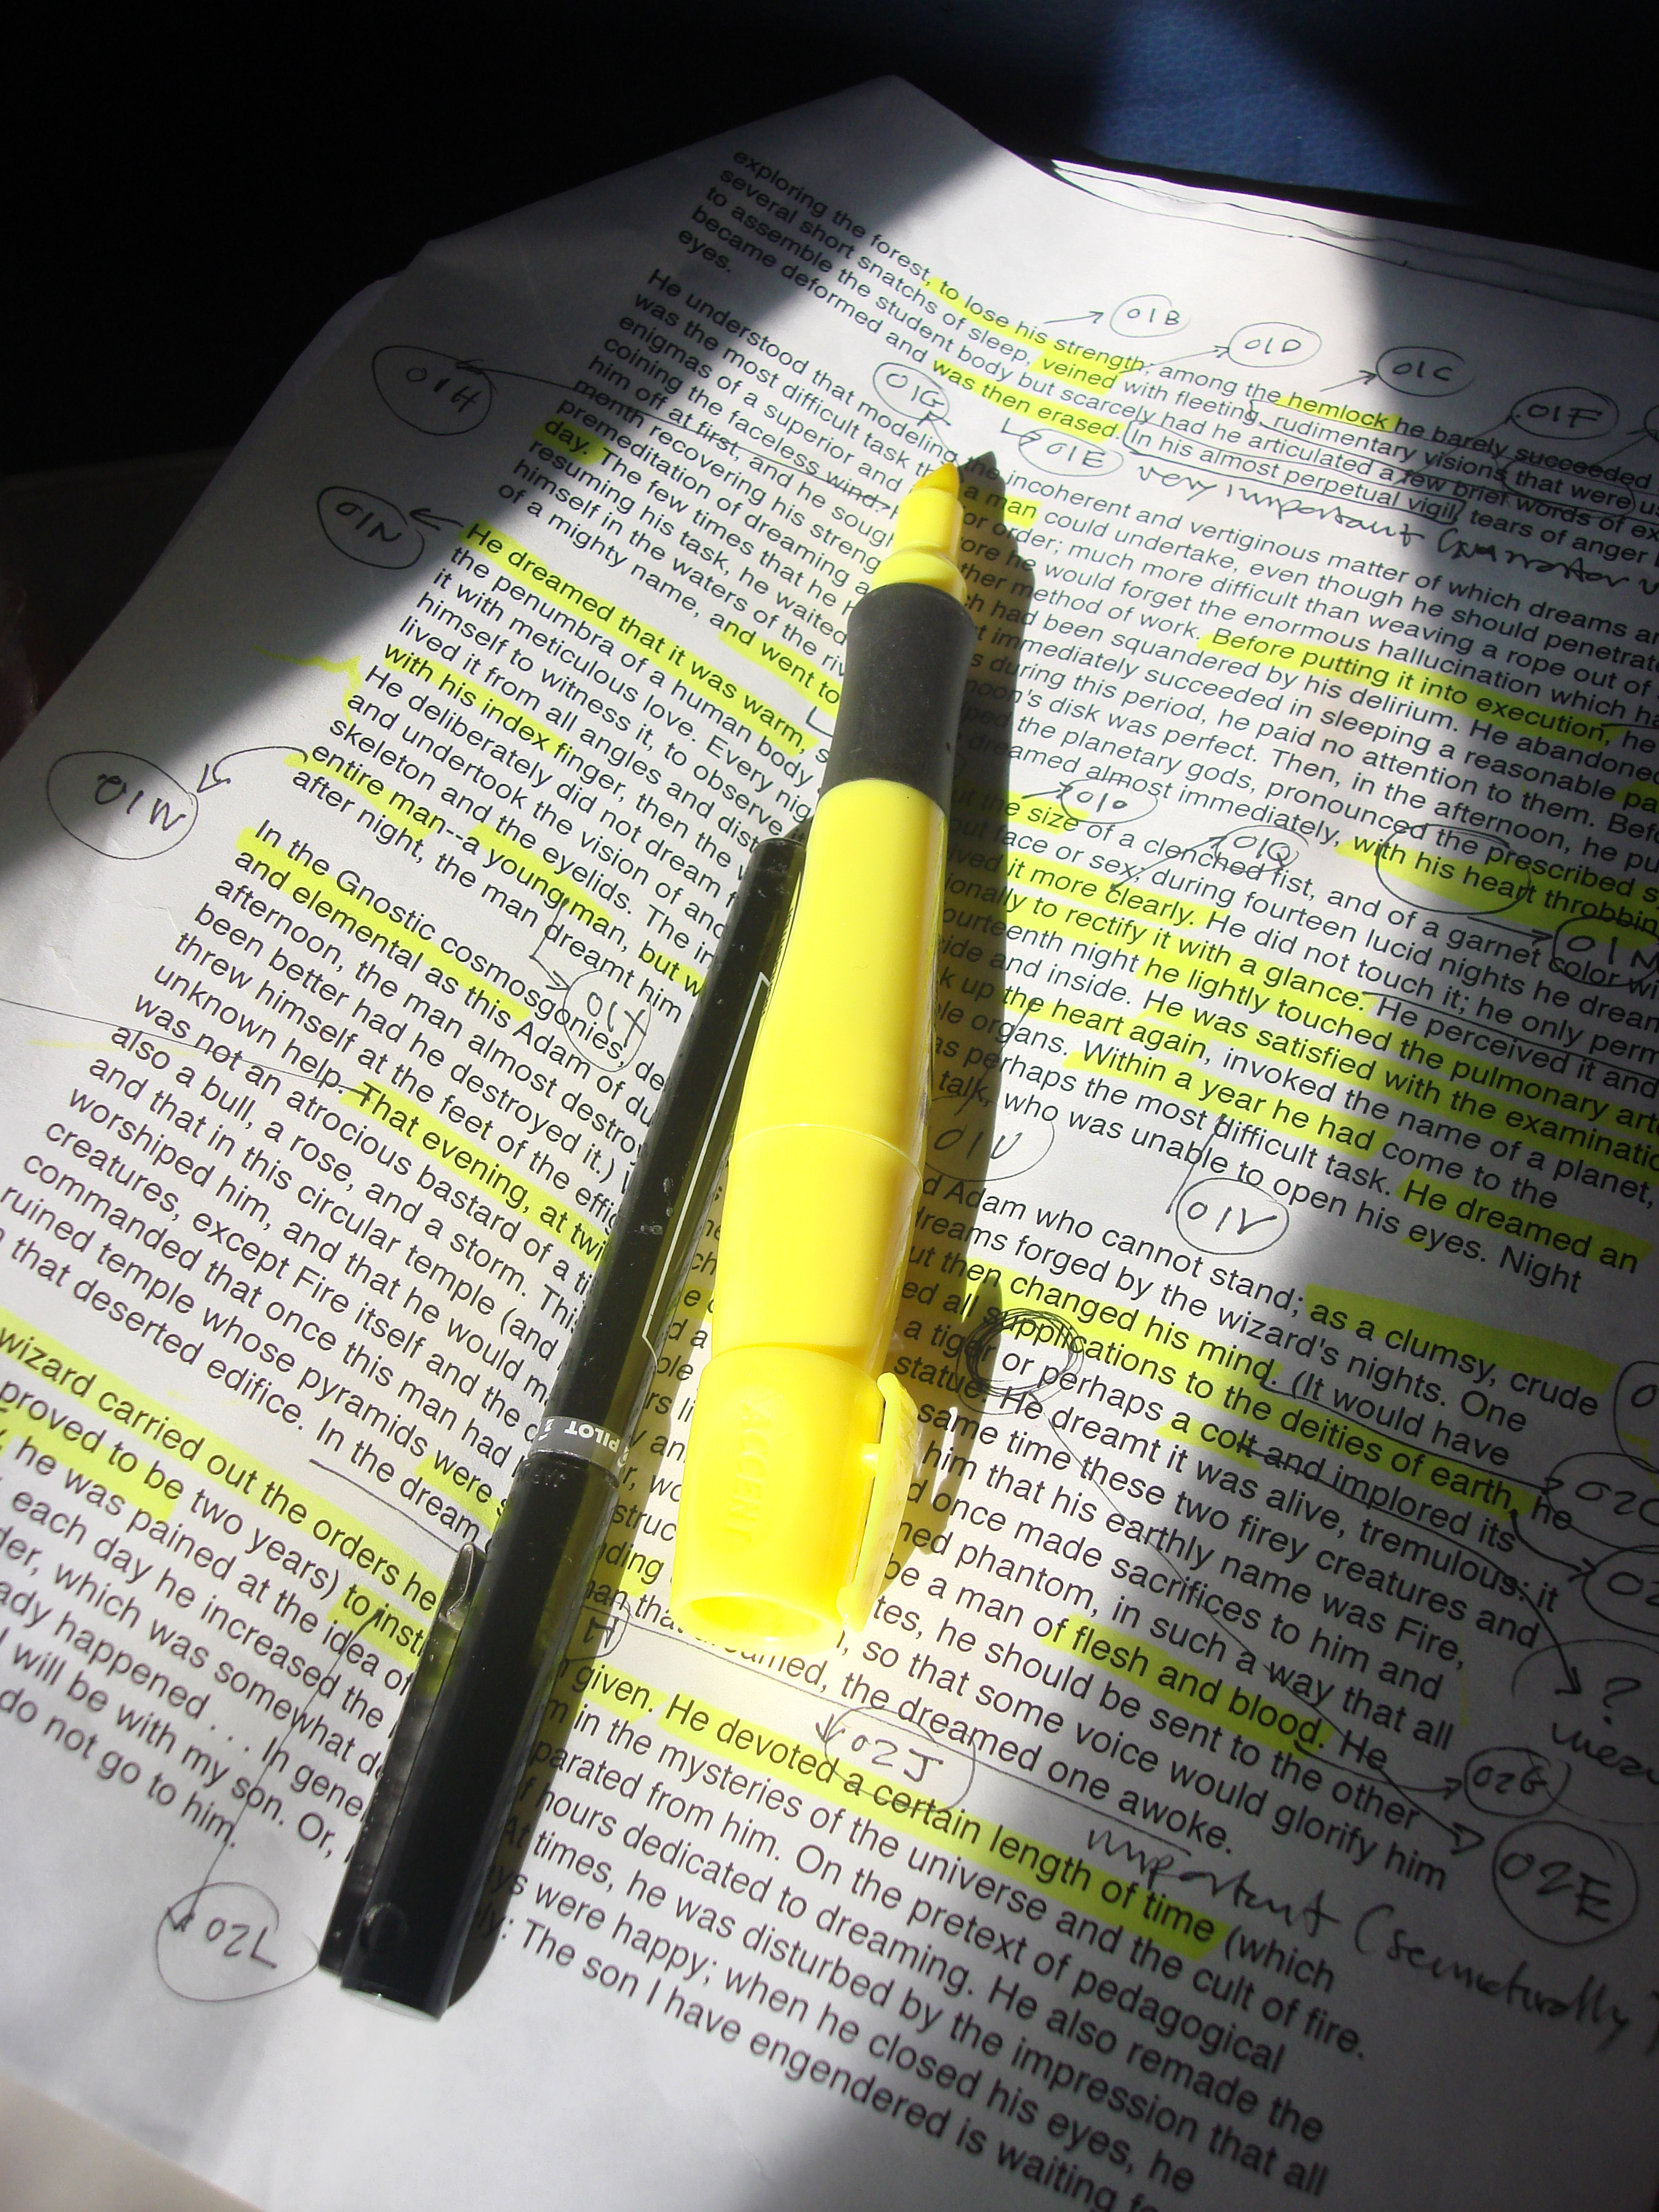
\includegraphics[width=\textwidth]{../img/textmarker}
  \end{columns}

  \vfill

  \hrulefill\\
  \hfill {\tiny Image by Guido ``random'' Alvarez, released as CC-BY-2.0}

\end{frame}

\subsection{Task 2: Understanding the Input/Output}

\begin{frame}
  \frametitle{Task 2: Reading the Input/Output}

  The Input Description is \alert{very important} (as we saw in 3n+1)

  \bigskip

  {\small
  \begin{itemize}
  \item What is the size of the data?
  \item What are the limits of the data?
  \item What is the format of the data?
  \item What is the stop condition?
  \end{itemize}
  }
\end{frame}

\begin{frame}
  \frametitle{Task 2: Input Size}

  The input size shows how big the problem gets.

  \begin{itemize}
  \item Small Problem: Full Search; Simulation;
  \item Big Problem: Complex Algorithms; Pruning;
  \end{itemize}

  \begin{block}{Keep in Mind!}
    \begin{itemize}
    \item The average time limit in UVA is 1-3 seconds.
    \item Expect maybe 10.000.000 operations per second.
    \end{itemize}
  \end{block}
\end{frame}

\begin{frame}
  \frametitle{Task 2: Input Size -- Examples}

  \begin{block}{n $<$ 24}
    Exponential algorithms will work (O($2^n$)).\\
    Or sometimes you can just calculate all solutions.
  \end{block}

  \begin{block}{n = 500}
    Cubic algorithms don't work anymore (O($n^3$) = 125.000.000)\\
    Maybe O($n^2\text{log}n$) will still work.
  \end{block}

  \begin{block}{n = 10.000}
    A square algorithm (O($n^2$)) might still work.\\
    But beware any big constants!
  \end{block}

  \begin{block}{n = 1.000.000}
    O($n$log$n$) = 13.000.000\\
    We might need a linear algorithm!
  \end{block}
\end{frame}

\begin{frame}
  \frametitle{Task 2: Input Format}

  Three common patterns for input format:
  \vfill

  \begin{itemize}
  \item Read $N$, then read $N$ queries;
  \bigskip

  \item Read until a special condition;
  \bigskip

  \item Read until EOF;
  \end{itemize}
\end{frame}

\begin{frame}[fragile]
  \frametitle{Task 2: Input Format}
  \begin{block}{}
    Read $N$, and then read $N$ queries;
    \bigskip

    Remember $N$ when calculating the size of the problem!
  \end{block}
  Example: \structure{Cost Cutting}

{\smaller
\begin{verbatim}
#include <iostream>
using namespace std;

int main()
{
    int n;
    cin >> n;

    for (; n > 0; n--)
    {
       // Do something
    }
}
\end{verbatim}}

\end{frame}

\begin{frame}[fragile]
  \frametitle{Task 2: Input Format}
  \begin{block}{}
    Read Until a Special Condition.

    Be careful: You can have \alert{many} queries before the condition!
  \end{block}

  Example: \structure{Request for Proposal:}\\
  The input ends with a line containing two zeroes.

{\smaller
\begin{verbatim}
int main()
{
   cin >> n >> p;
   while (n!=0 || p!=0)
   {
       // do something!
       cin >> n >> p;
   }
}
\end{verbatim}}
\end{frame}

\begin{frame}[fragile]
  \frametitle{Task 2: Input Format}
  \begin{block}{}
    Read until EOF.
    \bigskip

    Functions in C and Java return FALSE when they read EOF. Python requires
    an exception. Very common in UVA.
  \end{block}
  Example: \structure{3N+1 Problem, Jolly Jumpers}

{\smaller
\begin{verbatim}
int main()
{
    int a, b;
    while (cin >> a >> b;)
    {
        // Do something!
    }
}
\end{verbatim}
}
\end{frame}

\begin{frame}
  \frametitle{Task 2: Output Format}

  The UVA judge decides the result based on a simple \alert{diff}.
  \bigskip

  Be \alert{very careful} that the output is exactly right!

  \vspace{3cm}

  \begin{columns}
    \column{0.2\textwidth}
    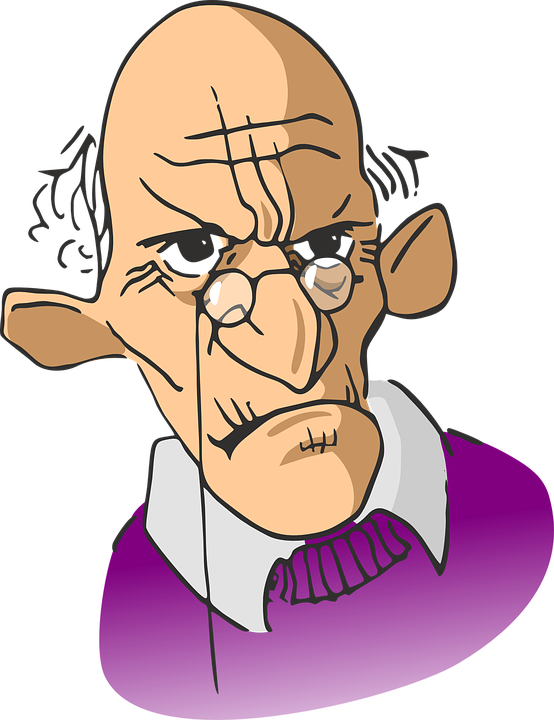
\includegraphics[width=1\textwidth]{../img/angryclient}
    \column{0.7\textwidth} \emph{The Judge is like an angry client. It
      wants the output EXACTLY how it stated.}
  \end{columns}
\end{frame}

\begin{frame}
  \frametitle{Task 2: Output Format -- Checklist}

  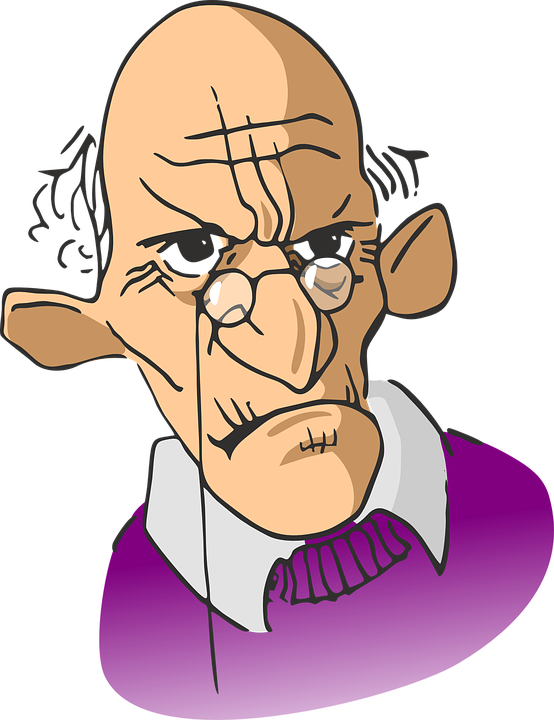
\includegraphics[width=0.15\textwidth]{../img/angryclient}
  \begin{enumerate}
    \item DID YOU REMOVE DEBUG OUTPUT?
    \item DID YOU REMOVE DEBUG OUTPUT?
    \smallskip

    \item Easy mistakes: UPPERCASE x lowercase, spleling mitsakes;
    \item Boring mistakes: plural: 1 hour \structure{or} 2 hours;
    \item What is the precision of \structure{float}? (3.051 \structure{or} 3.05)
    \item Round up or Round down? (3.62 $\rightarrow$ 3 \structure{or} 4)
    \item Multiple solutions: Which one do you output\\ (usually ortographical sort)
  \end{enumerate}
\end{frame}


\begin{frame}
  \frametitle{Task 2: Input/Output -- Traps!}

  \begin{block}{Example: 3n+1 Problem}
    \begin{itemize}
    \item $i$ and $j$ can come in any order.
    \end{itemize}
  \end{block}

  \begin{block}{Common Traps}
    \begin{itemize}
    \item Negative numbers, zeros;
    \item Duplicated input, empty input;
    \item No solutions, multiple solutions;
    \item Other special cases;
    \end{itemize}
  \end{block}
  \vfill

  \hfill 
\includegraphics[width=0.25\textwidth]{../img/trap}
\end{frame}

\subsection{Task 3: Choosing the algorithm}


\begin{frame}
  \frametitle{Task 3: Choosing the algorithm}
  The important part of choosing the algorithm is \alert{counting the time}
  \bigskip

  \begin{itemize}
    \item An algorithm with $k$-nested loops of and $n$ commands
      has $O(nk)$ complexity;
    \item A recursive algorithm with $b$ recursive calls per level, and $L$
      levels, it should have $O(bL)$ complexity;
    \item An algorithm with $p$ nested loops of size $n$ is $O(n^p)$
    \item An algorithm processing a $n*n$ matrix in O(k) per cell runs
      in $O(kn^2)$ time.
  \end{itemize}

  \bigskip

  Use \alert{pruning} to reduce the complexity of your algorithm!\\
  Also don't forget the number of queries!
\end{frame}

\begin{frame}[fragile]
  \frametitle{Task 3: Example of Pruning -- 8 queen problem}

  \hfill 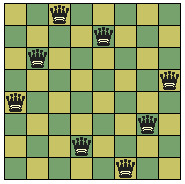
\includegraphics[width=0.2\textwidth]{../img/8queen}

  You want to find a position for 8 queens where no queen attack another queen.

  \bigskip

\begin{verbatim}
Solution 1: All options:
Queen1: a1 or a2 or a3 or a4 ... or h5 or h6 or h7 or h8
Queen2: Same as Queen 1
Queen3: Same as Queen 2
...
Queen8: Same as Queen 7

Total Solutions: 64 x 64 x 64 x 64 = 64^8 ~ 10^14
\end{verbatim}
\end{frame}

\begin{frame}[fragile]
  \frametitle{Task 3: Example of Pruning -- 8 queen problem}

  \hfill 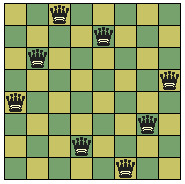
\includegraphics[width=0.2\textwidth]{../img/8queen}

  You want to find a position for 8 queens where no queen attack another queen.

  \bigskip

\begin{verbatim}
Solution 2: One queen / column
Queen1: a1 or a2 or a3 ...
Queen2: b1 or b2 or b3 ...
Queen3: c1 or c2 or c3 ...
...
Queen8: h1 or h2 or h3 ...

Total Solutions: 8 x 8 x 8 ... = 8^8 ~ 10^7
\end{verbatim}
\end{frame}

\begin{frame}[fragile]
  \frametitle{Task 3: Example of Pruning -- 8 queen problem}

  \hfill 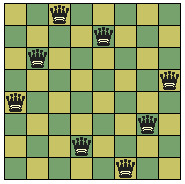
\includegraphics[width=0.2\textwidth]{../img/8queen}

  You want to find a position for 8 queens where no queen attack another queen.

  \bigskip

\begin{verbatim}
Solution 3: One queen / row x column
If Q1 is a1, Q2 in b2, Q3 must be c3-7...

A solution is the order of rows: Ex: 1-3-5-2-7-4-8-6

Total Solutions: 8 x 7 x 6 x 5 ... = 40320
\end{verbatim}
\end{frame}

\subsection{Task 4: Coding}

\begin{frame}
  \frametitle{Task 4: Coding}

  Do you understand \structure{The Problem} and \structure{The Algorithm}?

  \bigskip

  {\bf NOW} you can start writing your program.

  \vfill

  \begin{block}{}
    If you start your program before you understand the solution, you
    will create many more bugs.
  \end{block}
\end{frame}

\begin{frame}
  \frametitle{Task 4: Coding}
  \begin{exampleblock}{Hint 1: ``The Library''}
    Create a file with code examples that you often use.
    \begin{itemize}
    \item Input/output functions;
    \item Common data structures;
    \item Difficult algorithms;
    \end{itemize}
   \end{exampleblock}

   \begin{block}{Hint 2: Use paper}
    \begin{itemize}
    \item Writing your idea on paper help you visualize;
    \item Sometimes you can find bugs this way;
    \end{itemize}
  \end{block}
\end{frame}

\begin{frame}
  \frametitle{Task 4: Coding}

  \begin{block}{Hint 3: Programmer Efficiency}
    Everyone knows about \structure{CPU efficiency} or
    \structure{Memory efficiency}.

    \bigskip

    But \structure{Programmer Efficiency} is very important too: Don't
    get \structure{tired/confused!}
  \end{block}

  \vfill

  \begin{itemize}
  \item Use standard library and macros;
  \item Your program just need to solve THIS problem;
  \item Use simple structures and algorithms;
  \item TDD mindset;
  \end{itemize}
\end{frame}


\subsection{Testing}
\begin{frame}
  \frametitle{Task 5,6: Test and Hidden Data}

  The example data {\bf is not} all the data!

  \bigskip

  \begin{columns}
    \column{0.45\textwidth}
    \begin{exampleblock}{Example Data}
      \begin{itemize}
      \item Useful to test input/output;
      \item Read the example data to understand the problem;
      \end{itemize}
    \end{exampleblock}
    \column{0.45\textwidth}
    \begin{alertblock}{Hidden Data}
      \begin{itemize}
      \item Used by the UVA judge;
      \item Contain bigger data sets;
      \item Includes special cases;
      \end{itemize}
    \end{alertblock}
  \end{columns}

  \medskip

  Generate your own set of hidden data before submitting!
\end{frame}

\begin{frame}
  \frametitle{What data to generate?}

  \begin{itemize}
  \item Datas with multiple entries (to check for initialization);
  \item Datas with maximum size (can be trivial cases);
  \item Random data;
  \item Border cases (maximum and minimum values in input range);
  \item Worst cases (depends on the problem);
  \end{itemize}
\end{frame}

\begin{frame}
  \frametitle{The uDebug Website}

  \begin{center}
    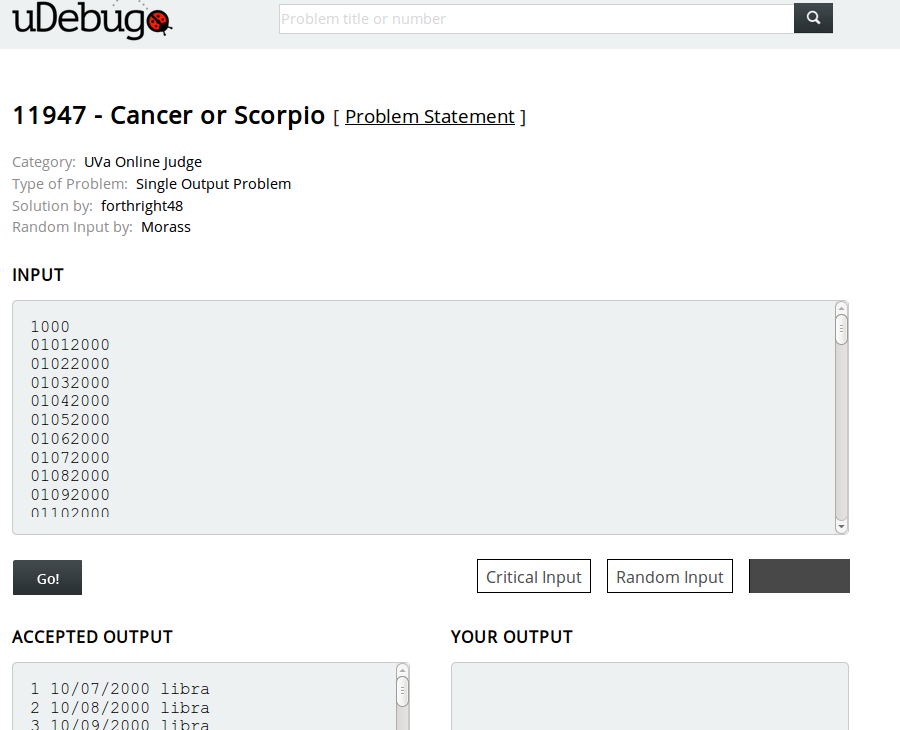
\includegraphics[width=0.8\textwidth]{../img/udebug_big}
  \end{center}
\end{frame}

\section{Conclusion}
\subsection{The End}
\begin{frame}
  \frametitle{To Summarize}
  Mental framework to solve problems:
  \begin{enumerate}
  \item Read the problem carefully to avoid traps;
  \item Think of the algorithm and data structure;
  \item Keep the size of the problem in mind;
  \item Keep your code simple;
  \item Create special test cases;
  \end{enumerate}

  \vfill

  \begin{block}{}
    Now go solve the other problems!
  \end{block}
\end{frame}

\begin{frame}
  \frametitle{Thanks for Listening!}
  \begin{center}
    Any questions?
  \end{center}
\end{frame}

\begin{frame}
  \frametitle{BONUS -- Calculating Complexity in Research Experiments}
\end{frame}

\begin{frame}
  \frametitle{BONUS -- A very simple program}

  \begin{block}{Ackermann's Function}
    \begin{eqnarray*}
      A(m,n) = & n+1 & \text{if } m = 0\\
      & A(m-1,1) & \text{if } m > 0, n = 0\\
      & A(m-1,A(m,n-1)) & \text{if } m > 0, n > 0\\
    \end{eqnarray*}
  \end{block}

  \begin{itemize}
    \item $A(0,n) = 1$ step
    \item $A(1,n) = 2n+2$ steps
    \item $A(2,n) = n^2$ steps
    \item $A(3,n) = 2^{n+3}-3$ \alert{!}
    \item $A(4,n) = 2^{2^{...^2}}-3$ \alert{!!!} (exponential tower of n+3)
    \item $A(5,n) = $ \alert{!!!!!!!!!!!!}
  \end{itemize}
\end{frame}
